\section{Introduction}
\label{sec:intro}

% Outline:
% - general intro statistical models of game outcomes
% - summarize our approach: skill-based, player kernel, bayesian
% - outline the paper

Statistical models of game outcomes have a rich and diverse history, going back almost a century:
as early as 1928, Zermelo \cite{zermelo1928berechnung} proposed a simple algorithm that infers the skill of chess players based on observed game outcomes.
Zermelo's ideas have since been rediscovered and refined multiple times, and have been successfully applied to various sports-related prediction problems and beyond.
On the occasion of the Euro 2016 football tournament, we revisit these ideas and highlight their connections to modern machine learning techniques.
In particular, we show how Zermelo's model can be cast as a Gaussian process classification model.
The Gaussian process framework provides two key advantages.
First, it brings all the benefits of Bayesian inference. In particular it provides a principled way to deal with the uncertainty associated to noisy observations and to predictions.
Second, it opens up new modeling perspectives through the specification of kernel functions.

Equipped with this, we investigate the problem of predicting outcomes of football matches between national teams.
We identify two key challenges,
\begin{enuminline}
\item that of \emph{data sparsity} (national teams usually play no more than ten matches per year), and
\item that of \emph{data staleness} (the team roster is constantly evolving).
\end{enuminline}
Taking inspiration from the observation that national teams' players frequently face each other in competitions between clubs (see Figure~\ref{fig:sankey}), we show that these two difficulties can be tackled by the introduction of a \emph{player kernel}.
This kernel relates any two matches through the players lined up on the field, and makes it possible to seamlessly use matches between clubs to improve a predictive model ultimately used for matches between national teams.
In contrast to national teams, clubs play much more frequently, and more data is available.

\begin{figure}[t]
  \centering
  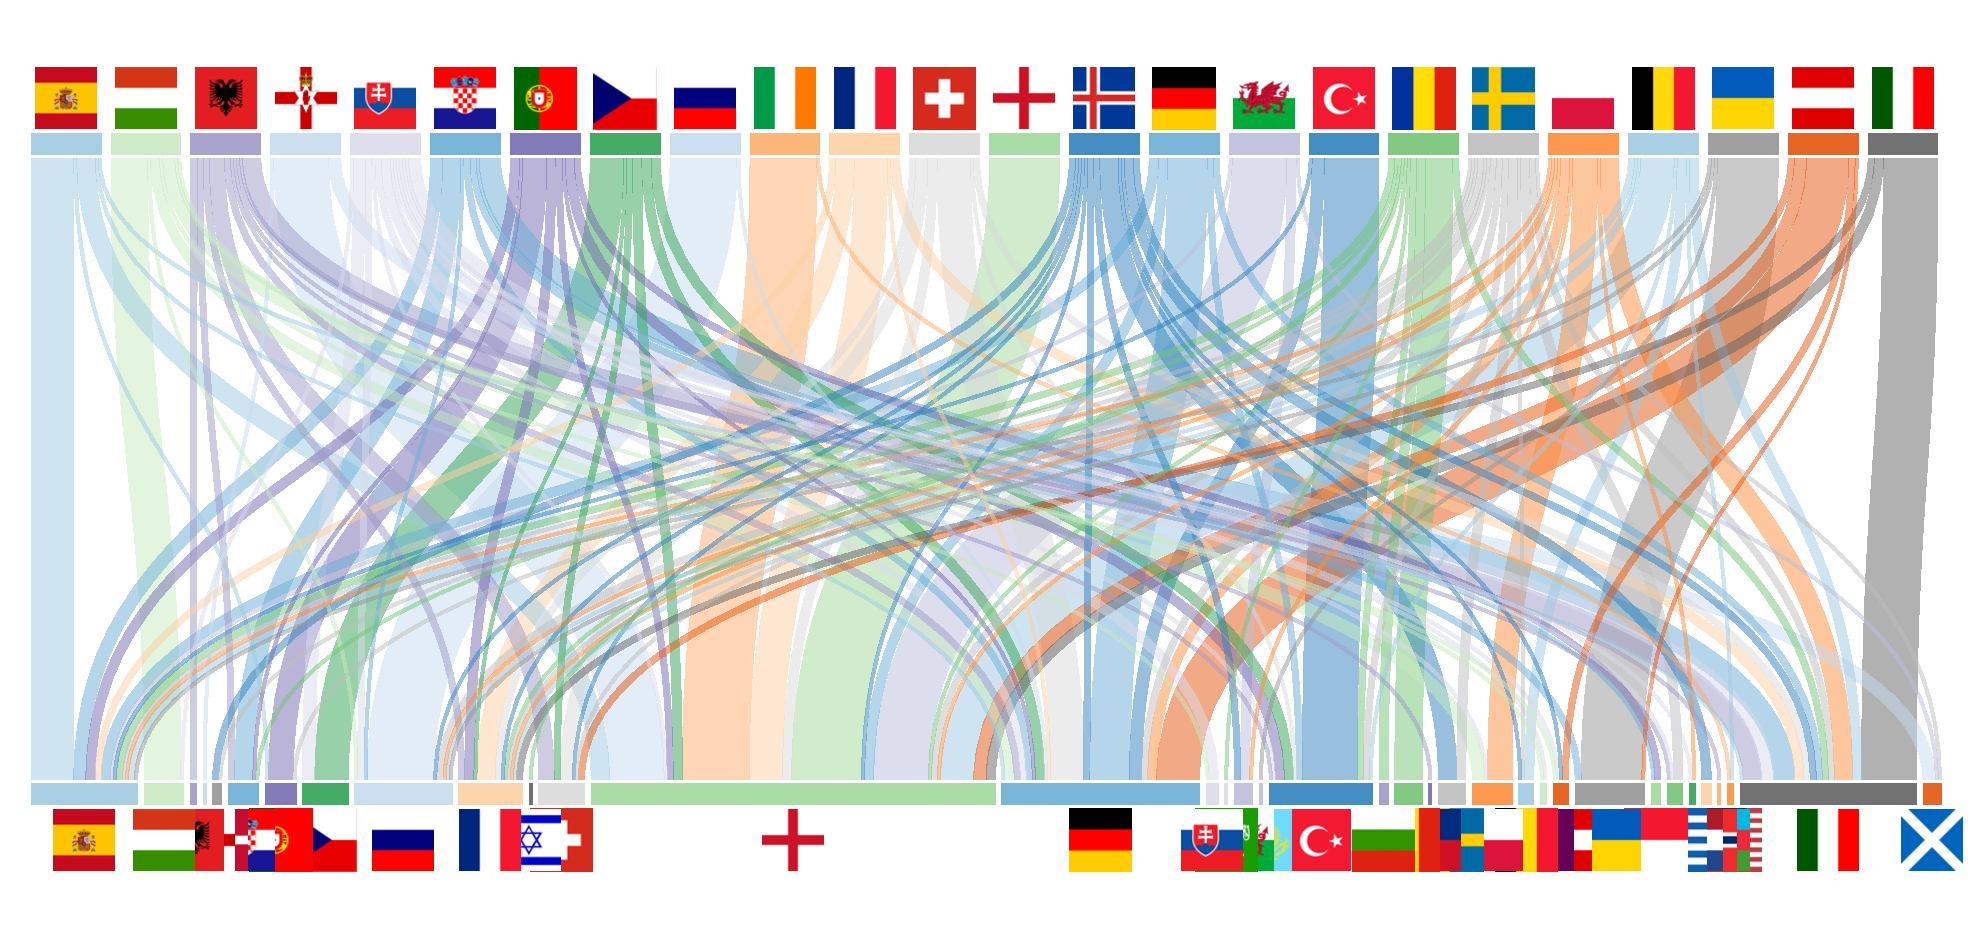
\includegraphics[width=\linewidth]{pk-sankey}
  \caption{
  Players of national teams qualified for the Euro 2016 (top row) are playing in clubs across Europe and beyond (bottom row).
  The English, German and Italian club championships contain the most selected players.
}
  \label{fig:sankey}
  \vspace{-0.1cm}
\end{figure}

The remainder of this short report is organized as follows.
We review related work at the end of the present section.
In Section~\ref{sec:methods}, we formalize the link between Zermelo's ideas and Gaussian processes, and present our player kernel.
Then, in Section~\ref{sec:evaluation}, we evaluate our predictive model on the Euro 2008, 2012 and 2016 final tournaments.


\subsection{Related Work}

More than two decades after Zermelo's seminal paper \cite{zermelo1928berechnung}, his model for paired comparisons was rediscovered and popularized by Bradley and Terry \cite{bradley1952rank}.
Nowadays, the model is usually referred to as the Bradley--Terry model.
In the context of skill-based game modeling, the same model (associated to a simple online stochastic gradient update rule) is also known as the Elo rating system \cite{elo1978rating}.
It is used by FIDE to rank chess players\footnote{See: \url{https://ratings.fide.com/}.} and by FIFA to rank women national football teams\footnote{See: \url{http://www.fifa.com/fifa-world-ranking/procedure/women.html}.}, among others.

The model and related inference algorithms have been extended in various ways; one direction that is of particular interest is the handling of uncertainty of the estimated skill parameters.
Glickman \cite{glickman1999parameter} proposes an extension that simultaneously updates ratings and associated uncertainty values after each observation.
Herbrich et al. \cite{herbrich2006trueskill} propose TrueSkill, a comprehensive Bayesian framework for estimating player skill in various types of games.
The models and methods described in this paper are fundamentally similar to TrueSkill, as will be discussed in Section~\ref{sec:methods}.
Finally, in the context of learning users' preferences from pairwise comparisons, Chu and Ghahramani \cite{chu2005preference} present a Gaussian process approach that is comparable to our work.
